\section{(2.3)}

\textit{A second floor of an office building has been given below:}
\begin{figure}[H]
\centering
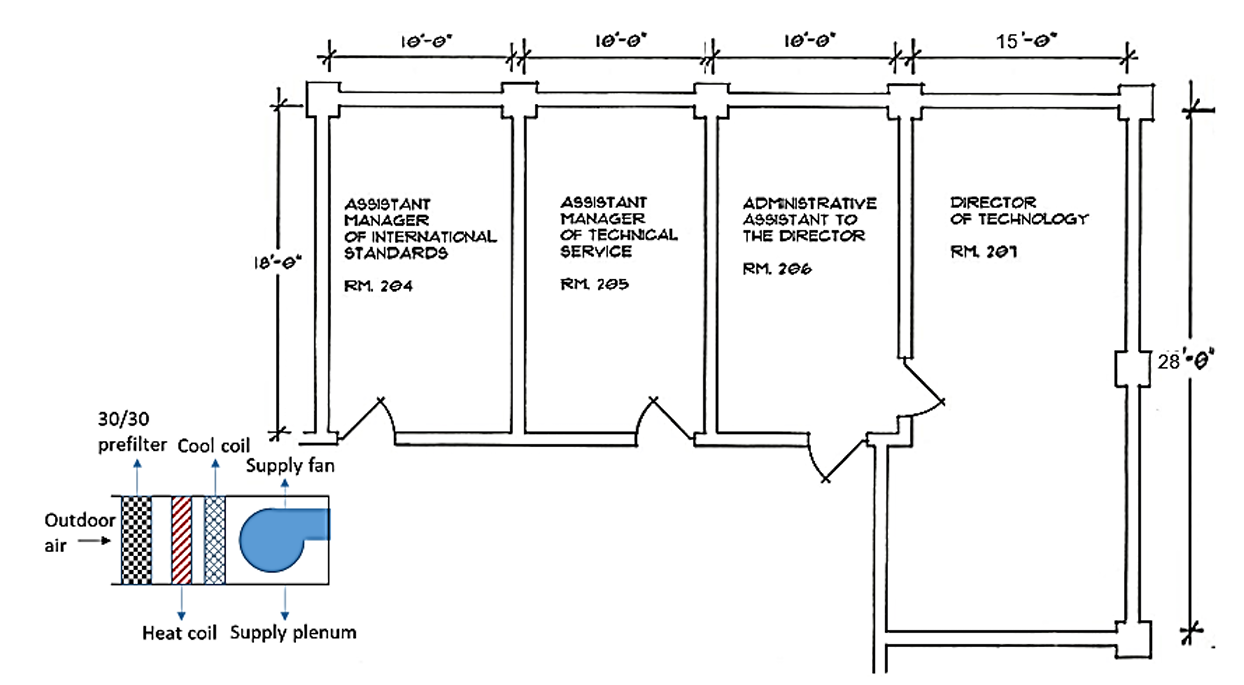
\includegraphics[width=0.9\textwidth]{Questions/Figures/Q1 Office Building.png}
\end{figure}
% An HVAC engineer has determined the amount of air per room (shown in the following table)
% required to maintain a comfortable and quiet space.
% Office Space Heating Air Requirement
% Office 204 330 cfm
% Office 205 470 cfm
% Office 206 190 cfm
% Office 207 520 cfm
% a) The architect has requested the design of a round ductwork system (duct material, sizes of round
% duct, necessary fittings, including diffusers, in a ductwork system, and the 2D system layout). You
% can use the dimensions of rooms to estimate the duct lengths. Note: You are free to design a duct
% system layout (No specific guidance needs to follow).
\textit{An HVAC engineer has determined the amount of air per room required to maintain a comfortable and quiet space}
\begin{table}[H]
\centering
\begin{tabular}{cc}
\toprule
Office Space & Heating Air Requirement (cfm) \\ 
\midrule
Office 204 & 330 \\
Office 205 & 470 \\
Office 206 & 190 \\
Office 207 & 520 \\
\bottomrule
\end{tabular}
\end{table}
\paragraph{a)} \textit{The architect has requested the design of a round ductwork system (duct material, sizes of round duct, necessary fittings, including diffusers, in a ductwork system, and the 2D system layout). You can use the dimensions of rooms to estimate the duct lengths. Note: You are free to design a duct system layout (No specific guidance needs to follow).}\\
\subsection{Assumptions:}
\begin{enumerate}
    \item $v_{\text{max}} = 1200$ fpm since the air is to be quiet for the office space.
    \item Round ductwork system
    \item $\Delta P$ unknown $\to$ friction loss = 0.1'' wg/100 ft.
    \item Diffusers are to be placed in each room. Assume that the pressure loss across the diffuser is 0.05'' wg. (Table 2.2).
    \item Galvanized steel duct material is used (common in air ducts).
    \item Bellmouth entrance from supply fan and diffuser entrance are to be considered.
    \item The elbow is pleated 90$^\circ$.
\end{enumerate}

\subsection{Sketches} 
Let us draw a sketch of a possible ductwork system layout for the office building.
\begin{figure}[H]
\centering
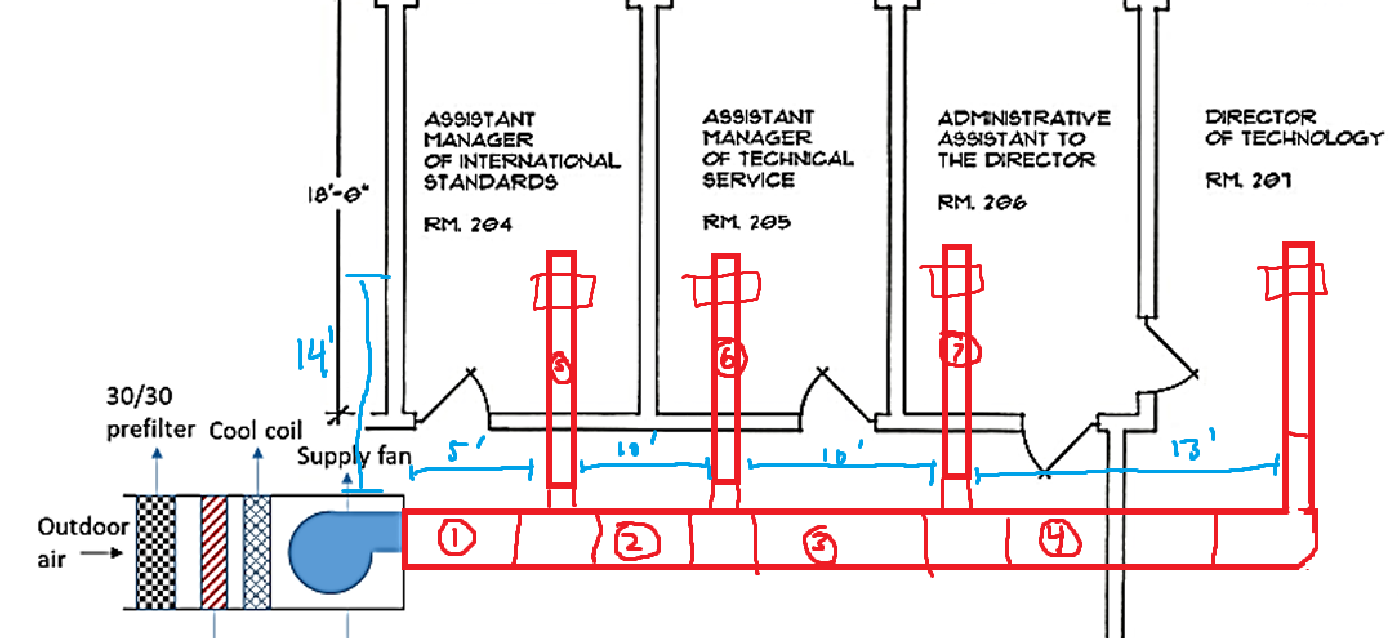
\includegraphics[width=0.9\textwidth]{Questions/Figures/Q1 Sketch.png}
\end{figure}

\subsection{Analysis}
\subsubsection{CFM in Sections}
Let us determine the required cfm for the differens sections. Based on the required cfm from the rooms, one can set:
\begin{table}[H]
\centering
\begin{tabular}{c c} \\
    \toprule
    Segment & Required cfm, $V_i$ \\
    \midrule
    5 & 330 \\
    6 & 470 \\
    7 & 190 \\
    4 & 520 \\
    \midrule \midrule
    3 & $V_7 + V_4$ = 710 \\
    2 & $V_6 + V_3$ = 1180 \\
    1 & $V_5 + V_2$ = 1510 \\
    \bottomrule
\end{tabular}
\end{table}
\subsubsection{Section Diameter}
Using the required cfm and the friction loss, the diameter of the ducts can be determined from the sizing chart:
\begin{figure}[H]
    \centering
    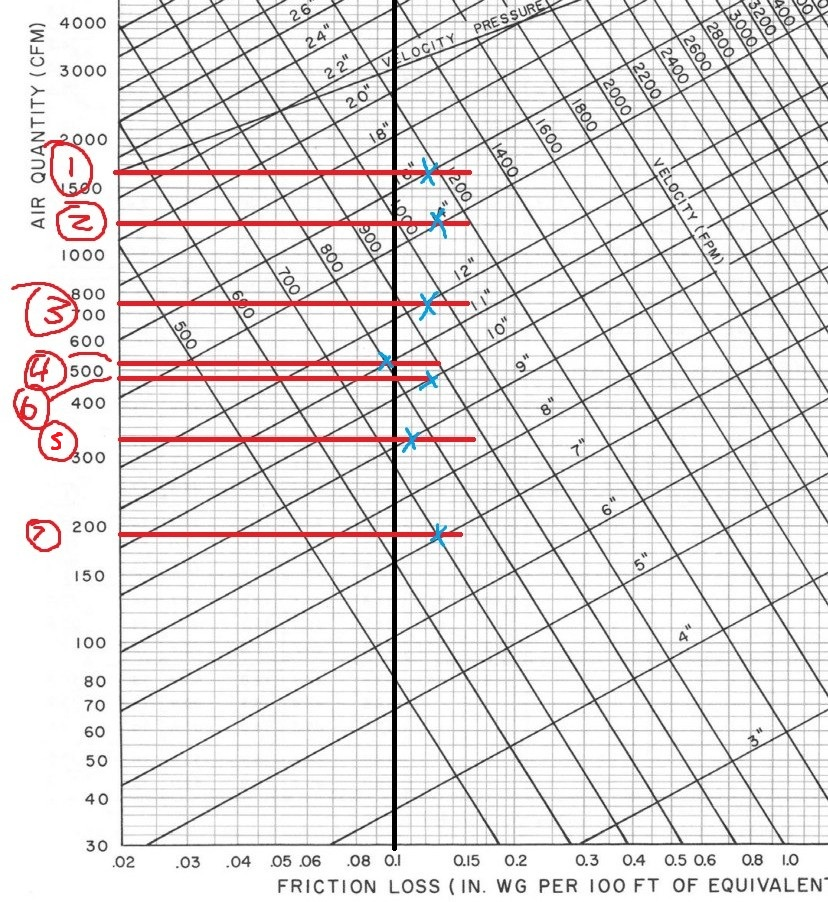
\includegraphics[width=0.7\textwidth]{Questions/Figures/Q1 Chart.jpg}
\end{figure}
In summary, 
\begin{table}[H]
\centering
\begin{tabular}{c c c c c} \\
    \toprule
    Segment & Required cfm & Diamter & Air Velocity fpm & Friction Loss ('' wg/100ft) \\
    \midrule
    1 & 1510 & 16'' & 1150 & 0.12 \\
    2 & 1180 & 14'' & 1100 & 0.13 \\
    3 & 710 & 12'' & 0950 & 0.12 \\
    4 & 520 & 11'' & 800 & 0.095 \\
    5 & 330 & 9'' & 750 & 0.11 \\
    6 & 470 & 10'' & 850 & 0.12 \\
    7 & 190 & 7'' & 700 & 0.13 \\
    \bottomrule
\end{tabular}
\end{table}

\subsection{Final Drawing}
\begin{figure}[H]
\centering
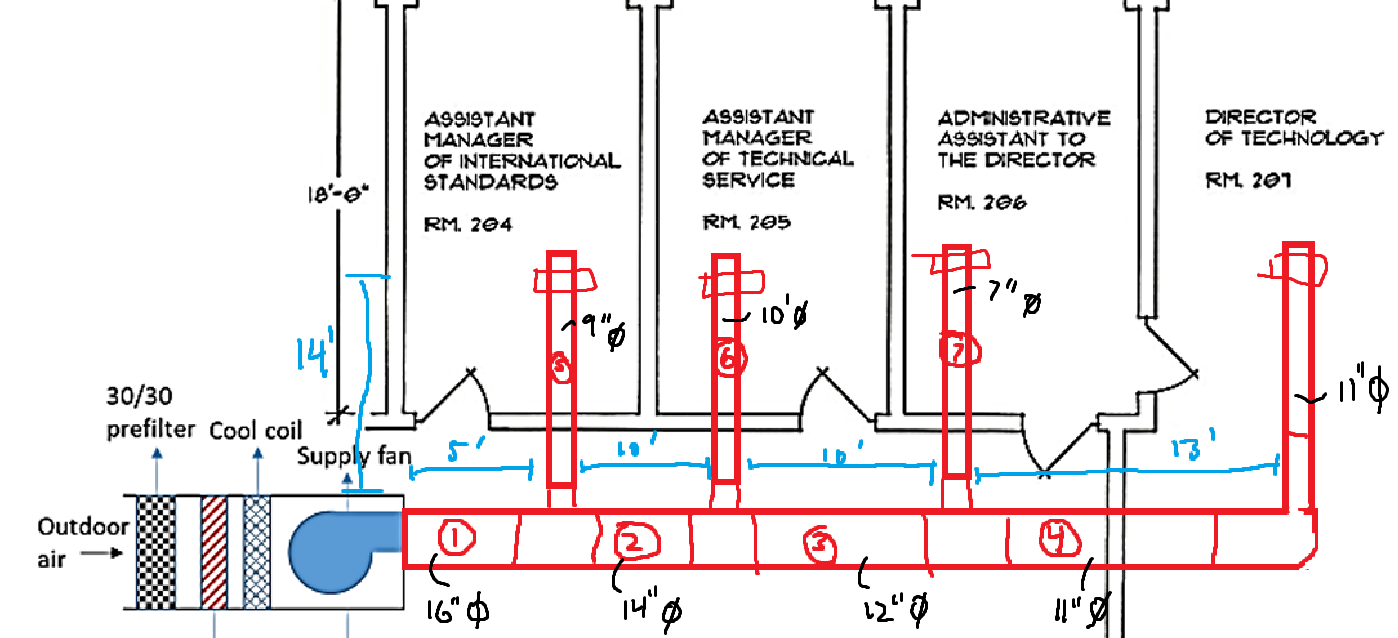
\includegraphics[width=0.9\textwidth]{Questions/Figures/Q1 Final Drawing.png}
\end{figure}

\subsection{Conclusion}
The system has been designed with round ducts with velocities that do not exceed the maximum velocity of 1200 fpm. The friction losses were within an acceptable range of 0.1'' wg/100 ft. The ducts were sized according to the required cfm and the pressure drop was calculated for each segment. The final drawing shows the layout of the ductwork system for the office building. Dampers can be added at the diffusers to balance the airflow in each room.

% Reset subsection counter
\newpage
\setcounter{subsection}{0}
\paragraph{b)} \textit{Based on the ductwork design, calculate the fan's minimum operating condition (airflow rate and static pressure). To be closer to reality, pressure losses from the air handling unit, including a prefilter, heating coils, cooling coils, and supply plenum, need to be considered in this project. The air handling unit is located in the bottom left corner, as indicated in this sketch.}\\
\subsection{Assumptions}
Assume Table 2.2 and A.4 are valid and applicable to the project.
\subsection{Analysis}
\subsubsection{Equivalent Lengths}
First determine the bellmouth equivalent lengths from Table A.4:
\begin{align*}
    L_{\text{BM}, 1} &= (16'') \cdot (12) = 192'' = 16' \\
    L_{\text{BM}, 5} &= (9'') \cdot (12) = 120'' = 9' \\
    L_{\text{BM}, 6} &= (10'') \cdot (12) = 120'' = 10' \\
    L_{\text{BM}, 7} &= (7'') \cdot (12) = 84'' = 7' \\
    L_{\text{BM}, 4} &= (11'') \cdot (12) = 132'' = 11' 
\end{align*}
Next, determine the tee equivalent lengths from Table A.4:
\begin{align*}
    L_{\text{(tee, thru,} 1)} &= (16'') \cdot (8) = 128'' = 10.67' \\
    L_{\text{(tee, thru,} 2)} &= (14'') \cdot (8) = 112'' = 9.33' \\
    L_{\text{(tee, thru,} 3)} &= (12'') \cdot (8) = 96'' = 8' \\
    L_{\text{(tee, thru,} 4)} &= (11'') \cdot (8) = 88'' = 7.33' \\
    L_{\text{(tee, branch,}5)} &= (9'') \cdot (8) = 72'' = 6' \\
    L_{\text{(tee, branch,}6)} &= (10'') \cdot (8) = 80'' = 6.67' \\
    L_{\text{(tee, branch,}7)} &= (7'') \cdot (8) = 56'' = 4.67' \\
\end{align*}
And lastly the elbow equivalent length from Table A.4:
\begin{align*}
    L_{\text{elbow, 90$^\circ$, 4}} &= (11'') \cdot (15) = 165'' = 13.75'
\end{align*}
The total equivalent for relevant sections are:
\begin{align*}
    L_{1\to2} &= L_{\text{BM}, 1} + L_{1} + L_{\text{(tee, thru,} 1)} \\
    &= 16' + 5' + 10.67' = 31.67' \\
    L_{2\to3} &= L_{2} + L_{\text{(tee, thru,} 2)} \\
    &= 14' + 9.33' = 23.33' \\
    L_{3\to4} &= L_{3} + L_{\text{(tee, thru,} 3)} \\
    &= 10' + 8' = 18' \\
    L_{2\to204} &= L_{\text{tee, branch,}5} + L_{5} + L_{\text{BM}, 5} \\
    &= 6' + 14' + 9' = 29' \\
    L_{3\to205} &= L_{\text{tee, branch,}6} + L_{6} + L_{\text{BM}, 6} \\
    &= 6.67' + 14' + 10' = 30.67' \\
    L_{4\to206} &= L_{\text{tee, branch,}7} + L_{7} + L_{\text{BM}, 7} \\
    &= 4.67' + 14' + 7' = 25.67' \\
    L_{4\to207} &= L_{4} + L_{\text{elbow, 90$^\circ$, 4}} + L_{4,h} + L_{\text{BM}, 4} \\
    &= 11' + 13.75' + 5' + 11' = 40.75' \\
\end{align*}
\subsubsection{Pressure Drop}
Converting to pressure drop:
\begin{align*}
    \Delta P_{1\to2} &= \frac{0.12}{100} \cdot 31.67 = 0.038\; \text{in-wg} \\
    \Delta P_{2\to3} &= \frac{0.13}{100} \cdot 23.33 = 0.030\; \text{in-wg} \\
    \Delta P_{3\to4} &= \frac{0.12}{100} \cdot 18 = 0.022\; \text{in-wg} \\
    \Delta P_{2\to204} &= \frac{0.11}{100} \cdot 29 = 0.032\; \text{in-wg} \\
    \Delta P_{3\to205} &= \frac{0.12}{100} \cdot 30.67 = 0.037\; \text{in-wg} \\
    \Delta P_{4\to206} &= \frac{0.13}{100} \cdot 25.67 = 0.033\; \text{in-wg} \\
    \Delta P_{4\to207} &= \frac{0.095}{100} \cdot 40.75 = 0.039\; \text{in-wg} 
\end{align*}
The pressure drop across the air handling unit can be calculated using Table 2.2:
\begin{align*}
    \Delta P_{\text{handling}} &=  \Delta P_{\text{plenum}} + \Delta P_{\text{filter}} + \Delta P_{\text{heating}} + \Delta P_{\text{cooling}} \\
    &= 0.50 + 0.30 + 0.35 + 0.35 = 1.50 \; \text{in-wg}
\end{align*}
The total pressure drop is:
\begin{align*}
    \Delta P_{\text{handling} \to 204} &= \Delta P_{1\to2} + \Delta P_{2\to204} + \Delta P_{\text{handling}} + \Delta P_{\text{diffuser}} \\
    &= 0.038 + 0.032 + 1.50 + 0.05 = 1.62 \; \text{in-wg} \\
    \Delta P_{\text{handling} \to 205} &= \Delta P_{1\to2} + \Delta P_{2\to3} + \Delta P_{3\to205} + \Delta P_{\text{handling}} + \Delta P_{\text{diffuser}} \\
    &= 0.038 + 0.030 + 0.037 + 1.50 + 0.05 = 1.65 \; \text{in-wg} \\
    \Delta P_{\text{handling} \to 206} &= \Delta P_{1\to2} + \Delta P_{2\to3} + \Delta P_{3\to4} + \Delta P_{4\to206} + \Delta P_{\text{handling}} + \Delta P_{\text{diffuser}} \\
    &= 0.038 + 0.030 + 0.022 + 0.033 + 1.50 + 0.05 = 1.67 \; \text{in-wg} \\
    \Delta P_{\text{handling} \to 207} &= \Delta P_{1\to2} + \Delta P_{2\to3} + \Delta P_{3\to4} + \Delta P_{4\to207} + \Delta P_{\text{handling}} + \Delta P_{\text{diffuser}} \\
    &= 0.038 + 0.030 + 0.022 + 0.039 + 1.50 + 0.05 = 1.68 \; \text{in-wg} \\
\end{align*}
\subsection{Conclusion}
The greatest pressure drop is through the air handling unit to Office 207. Therefore minimum operating condition for the fan is 1.68'' in. wg and 1510 cfm. 
\newpage